\documentclass[convert={density=400,size=640x480,outext=.png}]{standalone}
\usepackage{tikz}
\usetikzlibrary{calc}
\usepackage{hax}

\begin{document}
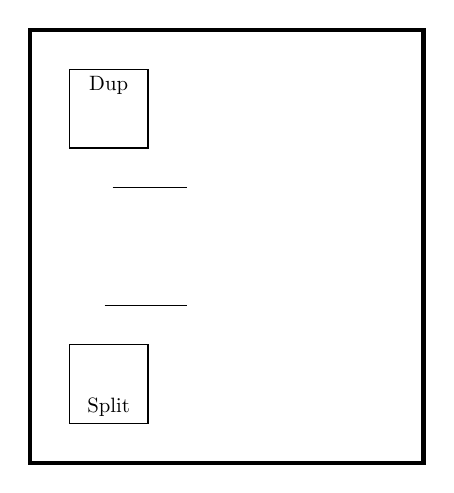
\begin{tikzpicture}[scale=0.5]
% lhs
\parser{(3,6)};
\parser{(3,11)};
% rhs
\parser{(15,6)};
\parser{(15,11)};
\draw [ultra thick] (11,12) rectangle (21,1);
% dup
\draw (12,11) rectangle (14,9);
\node [below, scale = 0.75] at (13,11) {Dup};
\blockoutput{(13.5,10)}{(14,10)};
\blockoutput{(12.9,9.5)}{(12.9,5)};
\draw (12.9,5) -- (15,5);
% split
\draw (12,4) rectangle (14,2);
\node [above, scale = 0.75] at (13,2) {Split};
\blockoutput{(13.5,3)}{(15,3)};
\blockoutput{(13.1,3.5)}{(13.1,8)};
\draw (13.1,8) -- (15,8);

\end{tikzpicture}
\end{document}